% --------------------------------------------------------------------------------

\begin{exercise}[Box of candles]

There are blue and red candles in a box.
Probability that a randomly chosen candle is blue is $\frac{1}{1 + 2 n}$, for $a > 0$.
Based on a sample of sample size $n$, find the maximum likelihood estimator (MLE) $\hat a$ of the parameter $a$.

\end{exercise}

% --------------------------------------------------------------------------------

\begin{solution}

The heavy lifting has already been done in \cite[lecture 6, slides 58-60]{EStat}.

\includepdf[
    pages = {58, 59, 60},
    nup = 1x2
]
{../../../EStat_VO/Lecture Slides/Lecture 6.pdf}

We only need to solve

\begin{align*}
    &
    \frac{1}{1 + 2 \hat a} \stackrel{!}{=} \hat p \\
    & \iff
    1 = \hat p (1 + 3 \hat a) = \hat p + 2 \hat a \hat p \\
    & \iff
    1 - \hat p = 2 \hat a \hat p \\
    & \iff
    \frac{1}{2}
    \pbraces
    {
        \frac{1}{\hat p} - 1
    }
    =
    \hat a.
\end{align*}

\end{solution}

% --------------------------------------------------------------------------------
